\documentclass[a4paper,12pt]{article}

% General document formatting
%\usepackage[margin=0.7in]{geometry}
\usepackage[parfill]{parskip}
\usepackage{url, hyperref}
\usepackage{color}
\usepackage[usestackEOL]{stackengine}[2013-10-15] % formatting Pascal
\usepackage[dvipsnames]{xcolor}

\usepackage{cancel}
\usepackage[export]{adjustbox}

% Related to math
\usepackage{amsmath,amssymb,amsfonts,amsthm}
\usepackage{mathtools}
\usepackage{youngtab}
\usepackage{tikz}

% encoding and language
\usepackage{lmodern}
\usepackage[slovene]{babel}
\usepackage[utf8]{inputenc}
\usepackage[T1]{fontenc}

% multiline comments
\usepackage{verbatim}

% images
\usepackage{graphicx}
\graphicspath{ {./images/} }

% theorems
\theoremstyle{definition}
\newtheorem{counter}{Counter}[section] % not for use
\newtheorem{defn}[counter]{Definicija}
\newtheorem{lemma}[counter]{Lema}
\newtheorem{conseq}[counter]{Posledica}
\newtheorem{claim}[counter]{Trditev}
\newtheorem{theorem}[counter]{Izrek}
\newtheorem{pro}[counter]{Dokaz}
%%
\theoremstyle{remark}
\newtheorem*{ex}{Primer}
\newtheorem*{rem}{Opomba}

% I like my squares DARK
\renewcommand\qedsymbol{$\blacksquare$}

% common commands redefined convenience purposes
\newcommand{\N}{\mathbb{N}}
\newcommand{\Z}{\mathbb{Z}}
\newcommand{\Q}{\mathbb{Q}}
\newcommand{\R}{\mathbb{R}}
\newcommand{\C}{\mathbb{C}}
\newcommand{\ch}{\operatorname{char}}

%%
\def\x{\hspace{3ex}}    %BETWEEN TWO 1-DIGIT NUMBERS
\def\y{\hspace{2.45ex}}  %BETWEEN 1 AND 2 DIGIT NUMBERS
\def\z{\hspace{1.9ex}}    %BETWEEN TWO 2-DIGIT NUMBERS
\stackMath

\begin{document}

\title{Kombinatorika - zapsiski s predavanj prof. Konvalinka}
\author{Domen Vogrin}
\author{Tomaž Poljanšek}
\date{jesen/zima 2021}
\maketitle


\pagenumbering{roman}
\tableofcontents
\newpage
\pagenumbering{arabic}


% date: 5. 10. 2021
\section{Osnovni principi kombinatorike}
\subsection{Funkcije in štetje}

\begin{defn}[Funkcija] \text{}

\begin{itemize}
\item injektivna (y je slika največ enega x) / ($x_1 \neq x_2 \rightarrow f(x_1) \neq f(x_2)$)
\item surj  ektivna (y je slika vsaj enega x) / ($\forall y \in Y \exists x \in X:f(x) = y$)
\item bijektivna /y je slika natanko enega x) / (injektivna in surjektivna)
\end{itemize}
\end{defn}

\[
\exists \ injektivnost: f: X\rightarrow Y: |X|\leqslant |Y|
\]
\[
\exists \ surjektivnost: f: X\rightarrow Y: |X|\geqslant |Y|
\]
\[
\exists \ bijektivnost: f: X\rightarrow Y: |X| = |Y|
\]

f: X $\rightarrow$Y lahko interpretiramo kot razporejanje kroglic (X) v škatle (Y).
Oznake:
\[
\N = \{0, 1, 2, ...\}
\]
\[
[n] = \{1, 2, ..., n\}
\]
\[
|[n]| = n
\]
\[
2^X = \{A\subseteq X\}  (= P(x))
\]
\[
Y^X = \{f: X\rightarrow Y\}
\]

Binomski izrek:
\[ \sum_{k=0}^{n}\binom{n}{k} x^k = (1+x)^n \]


\subsection{Dirichletovo načelo (princip)}
Če obstaja injektivna preslikava
\[
f: X\rightarrow Y \implies |X| \leqslant |Y|
\]
Ekvivalentno:
\[
|X| > |Y| \implies \neg \exists \ inj. \ f: X \rightarrow Y
\]
Ekvivalentno: \\
Če damo n kroglic v k škatel, n > k, sta v vsaj eni škatli vsaj dve kroglici.

\subsection{Načelo vsote in produkta}

\[
A \cap B = \emptyset
\]
\[
|A \cup B| = |A| + |B|
\]

V splošnem (načelo vključitev in izkjučitev):
\[
|A \cup B| = |A| + |B| - |A \cap B|
\]


Načelo produkta:
\[
|A\times B| = |A|\cdot|B|
\]

Kako uporabljamo ti dve načeli?
\begin{itemize}
\item načelo vsote: dve (disjunktni) možnosti, obarvamo vsako posebej, rezultata seštejemo
\item načelo produkta: naredimo dve \underline{neodvisni} izbiri, število možnosti za eno in drugo zmnožimo
\end{itemize}

\begin{claim}
$|2^X| = 2^{|X|}$
\end{claim}


\begin{pro}
 \ \\formalen:\\
\[\Phi = 2^X \rightarrow \{0, 1\}\times\{0, 1\}\times...\times\{0, 1\} \ (n-krat)\]
\[\Phi(A) = (\varepsilon_1, ..., \varepsilon_n), A \subseteq X\]
\[\varepsilon_i = \begin{cases}0: \quad x_i \notin A  \\ 1; \quad x_i \in A \end{cases}\]


\[
\Psi : \{0, 1\}^n \rightarrow 2^X
\]
\[
\Psi (\varepsilon_1, ..., \varepsilon_n) = \{x_i : \varepsilon_i = 1\}
\]


\[\Psi \circ \Phi = id_{2^X}\]
\[\Phi \circ \Psi = id_{\{0, 1\}^n}\]
\[\implies \Phi \text{ je bijekcija}\]
\[|\{0, 1\}^n| = 2^n \text{ po načelu produkta}\implies |2^X| = 2^{|X|}\]
\qed

Intuitivni dokaz:\\
za $\forall$ od n elementov imamo dve izbiri (damo / ne damo v podmn.), izbire so neodvisne, imamo
$2 \cdot 2 \cdot ...\cdot 2 = 2^n$
izbir.
\qed
\end{pro}

\begin{claim}
$|Y^X| = |Y|^{|X|}$
\end{claim}




\begin{pro}
\[\Phi : Y^X \rightarrow Y^{|X|}\]
\[X = \{x_1, ..., x_n\}\]
\[\Phi (f) = (f(x_1), ..., f(x_n))\]
\[\Psi (y_1, ..., y_n) = f\]
\[f(x_i) = y_i\]

Intuitivno:\\
Za vsak element iz X imamo |Y| izbir, izbire so neodvisne, torej imamo $|Y|\cdot|Y|\cdot ... \cdot|Y| = |Y|^{|X|}$ izbir.
\qed
\end{pro}

\begin{claim}
Število injektivnih preslikav v $Y^X$ je |Y| (|Y| - 1) ... (|Y| - |X|+1)
\end{claim}

\begin{pro}
Za sliko prvega elementa imamo |Y| izbir, za drugega (|Y| - 1) ...\\
Opomba: tu smo uporabili varianto pravila produkta - izbire niso neodvisne, je pa neodvisno število izbir.\\
Velja tudi za |X|$ > $|Y| (= 0)
\qed
\end{pro}

\subsection{Permutacije}

\begin{defn}
Bijektivna preslikava iz X samo vase se imenuje PERMUTACIJA. Množica permutacij:
\[S(x) = S_x\]
$S_n \coloneqq S([n]) $
\end{defn}

(Relacija R $\subseteq X\times Y , (x,y)\in R \ ali \ xRy)$

Relacija f je preslikava, če velja:
\[\forall x \in X \; \exists! y \in Y: xfy\]
Pišemo $y=f(x).$

\begin{claim}
\[|S_n| = n!\]
\end{claim}
\begin{pro}
Za sliko 1 imamo n možnosti, za sliko 2 (n - 1) možnosti ...
\qed
\end{pro}

%13. 10. 2021

Kompozicija:
\[426135 \cdot 361254 = 654231\]
je asociatovnoa, ni komutativna.\\
Enota:
\[id = 12...n\]
Inverz:
\[426135^{-1} = 425163\]

($S_n$, $\cdot$ ) je simetrična grupa.\\
 \\
Naj bo $\pi \in S_n, \ i \in [n]$
\[i, \pi (i), \pi^2(i), \pi^3(i), ...\]
Po Dirichletovem principu $\exists j, j', j < j': \pi^j(i) = \pi^{j'}(i) \implies i = \pi^{j'-j}(i)$
\[(i \ \pi(i) \ \pi^2(i) \ ... \ \pi^{n - 1}(i))\]
Permutacijo lahko zapišemo kot produkt disjunktnih ciklov
\[\pi = 426135 = (1 4)(2)(3 6 5)\]

\section{Podmnožice in načrti}
\subsection{Binomski koeficienti}

$2^A$ potenčna množica
\[2^A = \{B \subseteq A\}\]
\[\binom{A}{k} = \{B \subseteq A: |B| = k\} \ (A \ nad \ k)\]
$\binom{n}{k}$ binomski koeficient
\[\binom{n}{k} = |\binom{[n]}{k}|\]
(n nad k ("n choose k"))
\}\}
$\binom{n}{k}$ = število k-elementnih podmnožic množice z n elementi = število načinov, da izberemo k izmed n elementov.
\[\binom{[4]}{2} = \{\{1, 2\}, \{1, 3\}, \{1, 4\}, \{2, 3\}, \{2, 4\}, \{3, 4\}\}\]

\begin{claim}
\[\binom{n}{k}=\frac{n(n-1)...(n-k+1)}{k!}\]
$n^{\underline{k}}$ "n na k padajoče" = n(n-1)...(n-k+1)\\
$n^{\overline{k}}$ "n na k naraščajoče" = (n)(n+1)...(n+k-1)
\[\binom{n}{k} = \frac{n(n-1)...(n-k+1)}{k!} = \frac{n^{\underline{k}}}{k!} = \begin{cases}\frac{n!}{k!(n-k)!}: \quad 0 \leq k \leq n   \\ 0: \quad \text{sicer} \end{cases}\]
\end{claim}

\begin{pro}\mbox{}\\
1. način:\\
Izberemo k števil izmed n števil brez ponavljanja, vrstni red je pomemben.\\
Torej: izberemo k-terico različnih števil
\[n(n-1)...(n-k+1)\]
Po drugi strani: $\binom{n}{k}$ (izberemo k-elementno podmnožico v [n]), k! (izberemo vrstni red)
\[\implies \binom{n}{k} k! = n^{\underline{k}}\]
\[\implies \binom{n}{k} = \frac{n^{\underline{k}}}{k!}\]
\qed

2. način:\\
Če k < 0 ali k > n $\implies$ očitno $\binom{n}{k}$ = 0\\
n! ... število permutacij [n]\\
Vsako k-podmnožico dobimo k!(n-k)!-krat
\[\implies \frac{n!}{k! (n-k)!}\]
\qed
\end{pro}

\begin{claim}[Rekurzivna formula]
\[\binom{n}{k} = \binom{n-1}{k-1} + \binom{n-1}{k}\]
\end{claim}

\begin{pro}\mbox{}\\
1. način:\\
k-elementarno podmnožico [n]
\begin{itemize}
    \item vsebuje n ($\binom{n-1}{k-1}$ vsebuje k-1 element iz [n-1])
    \item ne vsebuje n ($\binom{n-1}{k-1}$ izmed n-1 izberemo k)
\end{itemize}
\qed

2. način:\\
\[\Phi : \binom{[n]}{k}\rightarrow \binom{[n - 1]}{k - 1} \cup \binom{[n - 1]}{k}\]
\[\Phi (A) = A \setminus \{n\}\]
\[\text{inverz}: \Psi(B) = \begin{cases}B \cup \{n\}: \quad |B| = k - 1 \\ B: \quad |B| = k \end{cases}\]
\qed

3. način:\\
\[\binom{n - 1}{k - 1}+\binom{n-1}{k} = \frac{(n-1)^{\underline{k-1}}}{(k-1)!} + \frac{(n-1)^{\underline{k}}}{k!} = \frac{(n-1)^{\underline{k-1}}(k+n-k)}{k!} = \frac{n^{\underline{k}}}{k!}, \ k \geqslant1\]
\qed
\end{pro}

\subsection{Pascalov trikotnik}

%(Image will be added soon (upam))
\Longstack[l]{
n=0\\
n=1\\
n=2\\
n=3\\
n=4\\
n=5\\
n=6\qquad\ \\
}
\Longstack{
1\\
1\x 1\\
1\x 2\x 1\\
1\x 3\x 3\x 1\\
1\x 4\x 6\x 4\x 1\\
1\x 5\y 10\z 10\y 5\x 1\\
1\x 6\y 15\z 20\z 15\y 6\x 1\\
\overline{0\x 1\x 2\x 3\x 4\x 5\x 6}
}


\subsection{Binomski izrek}
\begin{defn}
\[(a + b)^n = \sum_{k = 0}^{n}{\binom{n}{k} a^{n-k} b^k}\]
\end{defn}
\begin{pro}\mbox{}\\
1. način: (indukcija na n)\\
\[n = 0: OK (1 = \binom{0}{0} a^0b^0 = 1)\]
\[n - 1 \rightarrow n\]
\[(a+b)^n = (a+b)^{n-1}(a+b) = (\sum_{k=0}^{n-1} \binom{n-1}{k} a^{n-1-k}b^k)(a+b) =\]
\[ = \sum_{k=0}^{n-1} \binom{n-1}{k} a^{n-k}b^k + \sum_{k=0}^{n-1} \binom{n-1}{k} a^{n-1-k}b^{k+1} =\]
\[=_{k' = k + 1} \sum_{k=0}^{n-1} \binom{n-1}{k} a^{n-k}b^k + \sum_{k'=1}^{n-1} \binom{n-1}{k'-1} a^{n-k'}b^{k'} = \]
\[=_{k'=k} \sum_{k=0}^{n} {\binom{n-1}{k}a^{n-k} b^k} + \sum_{k=0}^{n} {\binom{n-1}{k-1}a^{n-k} b^k} =\]
\[= \sum_{k=0}^n (\binom{n-1}{k} + \binom{n-1}{k-1})a^{n-k}b^k =\]
\[=_{rekurzija} \sum_{k=0}^n \binom{n}{k}a^{n-k}b^k\]
\qed

2. način (isti!)\\
Namesto $\sum_{k=0}^{n-1}$ oz. podobno se uporabi kar $\sum_k$ - vsi ostali členi so po definiciji binomskih koeficientov enaki 0. Postopek je podoben, samo vse skupaj je malo hitreje, ker preskočimo vmesne razmiselke.
\qed

3. način: (boljši!)\\
\[(a+b) \cdot (a+b) \cdot... \cdot (a+b)\]
Po distributivnosti iz vsakega oklepaja izberemo a ali b. Če smo b izbrali k-krat, smo a izbrali (n-k)-krat in dobimo $a^{n-k}b^k$. Kolikokrat dobimo $a^{n-k}b^k$? $\binom{n}{k}$-krat, ker izberemo k oklepajev, v katerih izberemo b.
\qed
\end{pro}

% 19. 10. 2021

\subsection{Izbori}

Na voljo imamo b oštevilčenih kroglic. Na koliko načinov lahko izberemo k kroglic?\\
Ali dovolimo ponavljanje?\\
Je vrstni red pomemben?\\

\begin{tabular}{c|c|c}

 & s ponavljanjem & brez ponavljanja \\
\hline
vrstni red \underline{je} pomemben & $n^k$ & $n^{\underline{k}}$\\
\hline
vrstni red \underline{ni} pomemben & $\binom{n + k - 1}{k}$ & $\binom{n}{k}$
\end{tabular}

OP.: v prvi vrstici gre za VARIACIJE, v drugi pa za KOMBINACIJE\\

\[1 \leqslant i_1 \leqslant ... \leqslant i_k \leqslant n\]
Želimo prešteti rešitve tega sistema neenačb.\\
n = 4, k = 3
\[1 1 1 \ \ \ 1 2 3 \ \ \ 2 2 2 \ \ \ 2 4 4\]
\[1 1 2 \ \ \ 1 2 4 \ \ \ 2 2 3 \ \ \ 3 3 3\]
\[1 1 3 \ \ \ 1 3 3 \ \ \ 2 2 4 \ \ \ 3 3 4\]
\[1 1 4 \ \ \ 1 3 4 \ \ \ 2 3 3 \ \ \ 3 4 4\]
\[1 2 2 \ \ \ 1 4 4 \ \ \ 2 3 4 \ \ \ 4 4 4\]

Ideja:
\[j_1 = i_1, \ j_2 = i_2 + 1, \ j_3 = i_3 + 2, \ ..., \ j_k = i_k + k - 1 \]

\subsection{Kompozicije}
\begin{defn}

\end{defn}
Kompozicija naravnega števila n je $\lambda = (\lambda_1, ..., \lambda_l)$, $\lambda_i > 0$, da velja
\[\lambda_1 + \lambda_2 + ... + \lambda_l = n\]
Primer: (3, 1, 5, 2) je kompozicija števila 11.
\[\lambda_1, ..., \lambda_l \text{ .......... členi kompozicije}\]
\[l \text{ ................. dolžina kompozicije}\]
\[n \text{ ................. velikost kompozicije}\]

\begin{claim}
Obstaja $2^{n-1}$ kompozicij števila n (n $\geqslant 1$) in obstaja $\binom{n - 1}{k - 1}$ kompozicij števila n s k členi.
\end{claim}

\begin{pro}
Kompozicijo lahko predstavimo s k kroglicami in pregradami:
\[3 + 1 + 5 + 2:\text{   O O O|O|O O O O O|O O}\]
n - 1 prostorov za pregrado $\implies$ 2 izbiri za vsako pregrado ($\exists, \ \nexists$)\\
k - 1 pregrad na n - 1 mestih: $\binom{n - 1}{k - 1}$
\qed
\end{pro}

\begin{defn}
Šibka kompozicija\\
Šibka kompozicija števila n je $\lambda = (\lambda_1, ..., \lambda_l)$,
\[\lambda_i \geqslant 0, \ \lambda_1 + ... + \lambda_l = n\]
\end{defn}
Šibkih kompozicij števila n je $\infty$.
Primer: (0, 0, 3, 1, 0, 5, 0, 2).
\begin{claim}
Število šibkih kompozicij n s k členi je $\binom{n + k}{k - 1}$.
\end{claim}

\begin{pro}\mbox{}\\
1. način:\\
Štejemo rešitve $\lambda_1 + \lambda_2 + ... + \lambda_k = n, \ \lambda_1 \geqslant 0$.\\
\[\mu_i = \lambda_i + 1\]
\[\mu_1 + ... + \mu_k = n + k, \mu_i \geqslant 1\]
\[\binom{n+k}{k-1} \text{ je rešitev.}\]
\qed

2. način:\\
Šibko kompozicijo predstavino s kroglicami in pregradami.
\[0 + 0 + 3 + 1 + 0 + 5 + 0 + 2:\text{   ||O O O|O||O O O O O||O O}\]
Imamo n + (k - 1) objektov, izberemo položaje pregrad na $\binom{n + k - 1}{k - 1}$ načinov.\\
OP.: Kombinacije s ponavljanjem (n kroglic, izberemo jih k)\\
$x_i$ ... kolikokrat smo izbrali kroglico:
\[x_i \geqslant 0, \ \ \ \ i = 1, \ ..., \ n\]
\[x_i + x_2 + ... + x_n = k\]
$\equiv$ šibke kompozicije k z n členi = $\binom{k + n - 1}{n - 1} = \binom{n + k - 1}{k}$
\qed
\end{pro}

\subsection{Načelo vključitev in izključitev (NVI)}
(Dodaj sliko (2 množici))
\[|A \cup B| = |A| + |B| - |A \cap B|\]
(Dodaj sliko (3 množice))
\[|A \cup B \cup C| = |A| + |B| + |C| - |A \cap B| - |A \cap C| - |B \cap C| + |A \cap B \cap C|\]

\begin{theorem}[NVI]
\[|A_1 \cup ... \cup A_n| = \sum_{j = 1}^{n} (-1)^{j - 1} \sum_{1 \leqslant i_1 \leqslant ... \leqslant i_j \leqslant n}|A_{i_1} \cap A_{i_2} \cap ... \cap A_{i_j}|\]
\end{theorem}

$A_I := \displaystyle \bigcap_{i \in I} A_i$\\
$A_{\{1,4,6,7\}} = A_1 \cap A_4 \cap A_6 \cap A_7$
\[|\bigcup_{i = 1}^{n} A_i| = \sum_{\emptyset \neq I \subseteq [n]} (-1)^{|I| - 1} |A_i|\]
$A_1, ... A_n \subseteq A$\\
$A_{\emptyset} = \{a \in A : a \in A_i : za \forall i \in \emptyset \} = A$
\[|\bigcap_{i = 1}^n A_i^c| = |(\bigcup_{i = 1}^n A_i)^c| = |A| - |\bigcup_{i = 1}^n A_i| = |A_{\emptyset}|
\sum_{\emptyset \neq I \subseteq [n]} (-1)^{|I|} (A_I)\]

Torej:
\[|\bigcap_{i = 1}^n A_i^c|  = \sum_{I \subseteq [n]} (-1)^{|I|} |A_I|\]

\begin{lemma}[k $\geqslant$ 1]
\[\sum_{j = 0}^k (-1)^j \binom{k}{j} = 0\]
\end{lemma}

\begin{pro}[lema]
\[(1 + x)^n = \sum_{k = 0}^n \binom{n}{k} x^k\]
x = -1
\[(1 -1)^n = \sum_{j = 0}^k \binom{k}{j} x^j = 0\]
\qed
\end{pro}

OPOMBA: Lema pravi $\sum_{j sod} \binom{k}{j} = \sum_{j lih} \binom{k}{j}$ oziroma število sodih podmnožic = število lihih podmnožic.

\[\varphi: \{sode podmnožica [k]\} \rightarrow \{lihe podmnožice [k]\} \]
\[\varphi (S) = \begin{cases}S \setminus \{k\}: \quad k \in S  \\ S \cup \{k\}: \quad k \notin S \end{cases}\]

\begin{pro}[NVI]
\[a \in \bigcup_{i = 1}^{n} A_i \text{, a vsebovana v natanko k množicah}\]
Dokazati želimo, da je doprinos a-ju k vsoti na desni = 1.
\[k - \binom{k}{2} + \binom{k}{3} - ... + (-1)^{k-1} \binom{k}{k} = \sum_{j = 1}^{k} (-1)^{j - 1} \binom{k}{j} = - (\sum_{j = 0}^{k} (-1)^j \binom{k}{j} - 1) = 1\]
k ... doprinos v prvi vrstici\\
$\binom{k}{2}$ ... doprinos v drugi vrstici\\
$\displaystyle \sum_{j = 0}^{k} (-1)^j \binom{k}{j}$ = 0 (po lemi)
\qed
\end{pro}

\subsection{Eulerjeva funkcija $\varphi$ $(\phi)$}
\[\phi (n) = |\{i \in [n] : \gcd(i, n) = 1\}|\]
\begin{claim}
\[\sum_{a | n} \phi (a) = n\]
(= število števil med 1 in n, ki so tuje n)
\end{claim}

\begin{pro}\mbox{}\\
Zapišimo $\frac{1}{n}$, $\frac{2}{n}$, $\frac{3}{n}$, ..., $\frac{n}{n}$ in jih pokrajšajmo.

\[
\begin{tabular}{c c c c c c c c c c c c}

$\frac{1}{12}$ & $\frac{2}{12}$ & $\frac{3}{12}$ & $\frac{4}{12}$ & $\frac{5}{12}$ & $\frac{6}{12}$ & $\frac{7}{12}$ & $\frac{8}{12}$ & $\frac{9}{12}$ & $\frac{10}{12}$ & $\frac{11}{12}$ & $\frac{12}{12}$\\
\\
$\frac{1}{12}$ & $\frac{1}{6}$ & $\frac{1}{4}$ & $\frac{1}{3}$ & $\frac{5}{12}$ & $\frac{1}{2}$ & $\frac{7}{12}$ & $\frac{2}{3}$ & $\frac{3}{4}$ & $\frac{5}{6}$ & $\frac{11}{12}$ & $\frac{1}{1}$

\end{tabular}
\]

Ulomkov je n, imenovalci so delitelji števila n, števci so števila, ki so $\leqslant$ a in tuja proti a.
\[\sum_{a | n} \phi (a) = n\]
\qed
\end{pro}
$A$ = [n], n = $p_1^{\alpha_1} ... p_k^{\alpha_k}$, $\alpha_i$ > 0\\
$A_i$ = $\{$j $\in$ [n] : $p_i$ | j$\}$
\[|A_i| = \frac{n}{p_i}\]
\[|A_i \cap A_j| = \frac{n}{p_i p_j}\]
\[|A_I| = \frac{n}{\displaystyle \prod_{i \subseteq I} p_i}\]

\[\phi (n) = \sum_{I \subseteq [k]} (-1)^{|I|} \frac{n}{\displaystyle \prod_{i \in I} p_i}\]
k = 2
\[n (1 - \frac{1}{p_1} - \frac{1}{p_2} + \frac{1}{p_1 p_2}) = n (1 - \frac{1}{p_1})(1 - \frac{1}{p_2})\]
\[\phi (n) =_{\text{distributivnost}}  n (1 - \frac{1}{p_1})(1 - \frac{1}{p_2})...(1 - \frac{1}{p_k})\]

\[\phi (n) = n \displaystyle \prod_{p | n} (1 - \frac{1}{p}\]

%26. 10. 2021

\subsection{Multinomski koeficienti}
\[\binom{n}{k} \ = \ \frac{n!}{k! (n - k)!}\text{, } 0 \leqslant k \leqslant n\]
Imamo a enic in b ničel. Premešamo jih lahko na 
\[\binom{a + b}{a} = \binom{a + b}{b} = \frac{(a+b)!}{a!b!}\]
načinov.\\
\[a_1 \times 1, a_2 \times  2, ..., a_n \times n \text{        (11122333334)}\]
Premešamo jih lahko na 
\[\binom{a_1 + a_2 + ... + a_n}{a_1} \cdot \binom{a_2 + a_3 ... + a_n}{a_2} \cdot \binom{a_3 + a_4 + ... + a_n}{a_3} ...\]
 V prvem binomu izberemo enke, v drugem dvojke, v tretjem trojke ... To razpišemo kot
\[\frac{(a_1 + a_2 + ... + a_n)!}{a_1!(a_2 + a_3 + ... + a_n)!} \cdot \frac{(a_2 + a_3 + ... + a_n)!}{a_2!(a_3 + a_4 + ... + a_n)!} \cdot \frac{(a_3 + a_4 + ... + a_n)!}{a_1!(a_4 + a_5 + ... + a_n)!} ... \frac{(a_{n-1}+a_n)!}{a_{n-1}!a_n!} =\]
\[= \frac{(a_1 + a_2 + ... + a_n)!}{a_1!a_2!...a_n!} = \frac{(\displaystyle \sum_{i = 1}^n a_i)!}{\displaystyle \prod_{i = 1}^n a_i!} = \binom{a_1 + a_2 + ... + a_n}{a_1, a_2, ..., a_n}\]

Drug dokaz: dodamo indekse $1_1 1_2 1_3 2_1 2_2 3_1 3_2 3_3 3_4 3_5 4_1$. Premešamo na
\[\frac{(a_1 + a_2 + ... + a_n)!}{a_1!a_2!...a_n!}\]
načinov. (premešamo na $(a_1 + a_2 + ... + a_n)!$ načinov, z $a_i!$ izbrišemo indekse)\\
OP:
\[\binom{a+b}{a, b} = \frac{(a+b)!}{a!b!} = \binom{a+b}{a} = \binom{a+b}{b}\]

\begin{theorem}[Multinomski izrek]
\[(x_1 + x_2 + ... + x_n)^m = \sum_{(a_1, ..., a_n)_{\text{šibka kompozicija m}}} \binom{m}{a_1, ..., a_n} x_1^{a_1}...x_n^{a_n}\]
\end{theorem}

\begin{pro}
\[(x_1 + x_2 + ... + x_n)(x_1 + x_2 + ... + x_n)...(x_1 + x_2 + ... + x_n)\]
Iz vsakega oglepaja izberemo $x_i$, kar skupaj pride $x_1^{a_1} x_2^{a_2}...x_n^{a_n}$, pri čemer je $\displaystyle \sum_{i = 1}^n a_i$ = m, $a_i \geqslant 0$. Koeficient je očitno $\binom{a_1 + a_2 + ... + a_n}{a_1, a_2, ..., a_n}$.
\qed
\end{pro}
\hrule
$x_1 = x_2 = ... = x_n$
\[n^m = \sum_{(a_1, ..., a_n)_{\text{šibka kompozicija m}}} \binom{m}{a_1, ..., a_n}\]


\subsection{Načrti in t-načrti}
Podjetje proizvaja več različic izdelka, želi jih testirati pri potrošnikih. Vsak potrošnik mora testirati enako število različic, vsako različico mora testirati enako število potrošnikov.

\[1234, 1247, 1357, 2468, 3568, 5678\]
8 različic, 6 potrošnikov, vsak potrošnik testira 4, vsako različico testirajo 3 potrošniki.

\begin{defn}\mbox{}\\
B = \{$B_1$, ..., $B_b$\} je narčt s parametri (v, k $\lambda$), če so $B_1$, ..., $B_b \subseteq$ [v], $|B_1|$ = ... = $|B_b|$ = k, $\forall$ i $\in$ [v] se pojavi v natanko $\lambda$ množicah ($B_i$ blokih).
\end{defn}

Naš primer je načrt s parametri (8, 4, 3).

Narišemo tabelo
\begin{tabular}{c|c c c}
     & $B_1$ & ... & $B_b$ \\
\hline
     1 \\
     ...\\
     v
\end{tabular}
Kljukico damo tam, kjer je i $\in B_j$. V vsakem stolpcu tako dobimo k kljukic, skupaj k$\cdot$b, v vsaki vrstici dobimo $\lambda$ kljukic, skupaj $\lambda \cdot$v. $\implies$ k$\cdot$b = $\lambda \cdot$v
\[\implies b = \frac{\lambda v}{k}\]

Velja še b $\leqslant$ $\binom{v}{k}$
\[\frac{\lambda v}{k} \leqslant \frac{v!}{k! (v-k)!}\]
Pokrajšamo $\frac{v}{k}$ na obeh straneh neenačbe in dobimo
\[\lambda \leqslant \frac{(v - 1)!}{(k - 1)! (v - k)!} = \binom{v-1}{k-1}\]

\begin{theorem}\mbox{}\\
Načrt s parametri (v, k, $\lambda$) obstaja natanko tedaj, ko velja k | v$\lambda$ in $\lambda \leqslant \binom{v - 1}{k - 1}$
\end{theorem}

\begin{pro}\mbox{}\\
($\Rightarrow$) Že dokazano.\\
($\Leftarrow$) Izberemo $\frac{\lambda v}{k}$ k-elementnih podmnožic množice [v]. To lahko naredimo, ker je $\frac{\lambda v}{k} \leqslant \binom{v - 1}{k - 1} \frac{v}{k} = \binom{v}{k}$.\\

v = 8, k = 4, $\lambda$ = 3\\
\[\frac{\lambda v}{k} = 6  \Rightarrow 1234, 1356, 1567, 1568, 2356, 3457\]
To ni nujno načrt.
\[\lambda_i \text{ ... v koliko blokih je vsebovan i}\]
\[\lambda_1 = 4, \lambda_2 = 2, \lambda_3 = 4, \lambda_4 = 2, \lambda_5 = 5, \lambda_6 = 4, \lambda_7 = 2, \lambda_8 = 1\]
Naredimo isto tabelo kot prej in ugotovimo, da je $\lambda = \frac{\sum_{i = 1}^v \lambda_i}{v}$.\\
Če to ni načrt zagotovo obstajata i, j, da je $\lambda_i$ > $\lambda$ > $\lambda_j$.\\

Bloki so 4 tipov:
\begin{itemize}
    \item[(I)] vsebujejo i in j
    \item[(II)] vsebujejo i, ne pa j
    \item[(III)] vsebujejo j, ne pa i
    \item[(IV)] ne vsebujejo ne i ne j\\
\end{itemize}

Bloki tipa (I) in (IV) vsebujejo enako i-jev in j-jev.
\begin{itemize}
    \item[] $\lambda_i$ = blokov tipa I + II
    \item[] $\lambda_j$ = blokov tipa I + III
\end{itemize}
Sledi, da je več blokov tipa II kot III. Iz tega sledi, da obstaja blok tipa II, tako da po zamenjavi i z n ne dobimo že obstoječega bloka.\\
1234, 1356, $\textcolor{red}{2}$567, 1568, 2356, 3457\\
V splošnem: $\lambda_i -= 1, \lambda_j += 1$\\
Postopek ponovimo, dokler ni $\lambda_1 = \lambda_2 = ... = \lambda_6$
\[1234, 1\textcolor{red}{4}56, 2567, 1568, 2356, 3457\]
\[1234, 145\textcolor{red}{7}, 2567, 1568, 2356, 3457\]
\[1234, 1457, 267\textcolor{red}{8}, 1568, 2356, 3457\]
\[1234, 147\textcolor{red}{8}, 2678, 1568, 2356, 3457\]
kar je načrt.\\
Na vsakem koraku se zmanjša $\displaystyle \sum_{i = 1}^v (\lambda_i - \lambda)$ za 2, po končno korakih je to = 0 in dobimo načrt.
\qed
\end{pro}

\begin{defn}[t-načrt]\mbox{}\\
B = \{$B_1$, ..., $B_b$\} je t-narčt s parametri (v, k $\lambda_t$), če je $B_1$, ..., $B_b \subseteq$ [v], $|B_1|$ = ... = $|B_b|$ = k, vsaka t-elementna podmnožica [v] je vsebovana v točno $\lambda_t$ blokih.
\end{defn}
(1-načrt = načrt)
\[124, 137, 156, 235, 267, 346, 457\]
je 2-načrt (7, 3, 1)\\
OP: Tudi načrt s parametri (7, 3, 3) NI 3-načrt!!\\

Favnova ravnina:\\
(Image will be added soon (upam))


\begin{theorem}\mbox{}\\
Če je B t-načrt s parametri (v, k, $\lambda_t$), je tudi (t-1)-načrt s parametri (v, k, $\lambda_{t-1}$)
\[\lambda_{t-1} = \lambda_t \cdot \frac{v - t + 1}{k - t + 1}\]
\end{theorem}

\begin{pro}
S $\subseteq$ [v], |S| = t - 1\\
S vsebovana v $\lambda_s$ blokih.
Narišemo tabelo
\begin{tabular}{c|c c c c c}
     & $B_1$ & ... & j & ... & $B_b$ \\
\hline
     1 \\
     ...\\
     i & & & \checkmark\\
     ...\\
     v
\end{tabular}
, i $\notin$ S, S $\cup \{i\} \subseteq B_j$. Skupno je:\\
(stolpci)
\begin{itemize}
    \item S$\setminus B_j$: 0 kljukic
    \item S $\subseteq B_j$: $k-t+1$ kljukic
    \item[] skupaj: $\lambda_s (k-t+1)$
\end{itemize}
(vrstice)
\begin{itemize}
    \item i$\in S$: 0 kljukic
    \item i$\notin S$: $\lambda_t$ kljukic
    \item[] skupaj: $\lambda_t (v-t+1)$
\end{itemize}

\[\Rightarrow \lambda_s = \frac{(v - t + 1)\lambda_t}{k-t+1}\]
\qed
\end{pro}



\section{Permutacije, razdelitve, razčlenitve}
\subsection{Stirlingova števila prve vrste}
$\pi \in S_n$ lahko zapišemo kot produkt disjunktnih ciklov
\[1 4 6 3 5 8 2 7 = (1)(2 4 3 6 8 7)(5)\]

\begin{defn}\mbox{}\\
Stirlingovo število prve vrste c(n, k) je število permutacij v $S_n$, ki imajo k ciklov.
\end{defn}
Za c(n, k) ni 'lepe' formule. Vemo c(n, n) = 1, c (n, n-1) = $\binom{n}{2}$ (transpozicija), c(n, 0) = 0 (n > 0) oziroma 1, če je n = 0. Vemo tudi c(n, 1) = (n-1)!, c(n, k) = 0 za k > n ali k < 0 ter
\[\sum_k c(n, k) = n!\]

\begin{claim}[Rekurzivna zveza]
\[c(n, k) = c(n-1, k-1) + c(n-1, k)\cdot(n-1)\]
\end{claim}

\begin{pro}
Permutacije v $S_n$ s k cikli:
\begin{itemize}
    \item n negibna točka: c(n-1, k-1)
    \item n ni negibna točka: c(n-1, k)  $\cdot$ (n-1) ((izbrišem n, dobim permutacijo v $S_{n-1}$ s k cikli) $\cdot$ (vsako dobimo (n-1)-krat))
\end{itemize}
\qed
\end{pro}


% 2.11.2021 by Tomaž
%\begin{Tomaž}

Tabela Stirlingovih števil 1. vrste: \\

\begin{tabular}{l|llllll}
    n \textbackslash k & 0 & 1  & 2  & 3  & 4  & 5 \\
    \hline \\
    0 & 1 & 0  & 0  & 0  & 0  & 0 \\
    1 & 0 & 1  & 0  & 0  & 0  & 0 \\
    2 & 0 & 1  & 1  & 0  & 0  & 0 \\
    3 & 0 & 2  & 3  & 1  & 0  & 0 \\
    4 & 0 & 6  & 11 & 6  & 1  & 0 \\
    5 & 0 & 24 & 50 & 36 & 10 & 1
\end{tabular}

Opomba: konstruiramo tako, da najprej damo diagonalne elemente na 1, naddiagonalne na 0, 1. stoplec
na 0 (razen prvega, ki je že 1), za ostale pa uporabimo rekurzivno forumlo (seštejemo element levo
zgoraj in (n-1) krat zgornji)

\begin{claim}[Rekurzivna zveza]
    \[\sum_k c(n,k)x^k = x^{\overline{n}}\]
\end{claim}

\begin{pro}\mbox{}\\
    indukcija na n: \\
    \[n = 0: OK (1x^0 = x^0)\]
    \[n - 1 \rightarrow n\]
    \[x^{\overline{n}} = x^{\overline{n-1}}(x+n-1) = \sum_k c(n-1,k)x^k (x+n-1) =\]
    \[= \sum_k c(n-1,k)x^{k+1} + \sum_k c(n-1,k)x^k (n-1) = \]
    \[\sum_k c(n-1,k-1)x^{k} + \sum_k c(n-1,k)x^k (n-1) =\]
    \[= \sum_k c(n,k)x^k\]
    \qed
\end{pro}

Opomba: dokaz lahko tudi v obratni smeri \\
\[x \leftrightarrow -x\]
\[\sum_k c(n,k) (-1)^k x^k = (-x)^{\overline{n}}\]
\[\sum_k (-1)^{n-k} c(n,k) x^k = x^{\underline{n}}\]
$s(n,k) := (-1)^{n-k} c(n,k)$ predznačeno stirlingovo število prve vrste
\[\sum_k s(n,k) x^k = x^{\underline{n}}\]

\subsection{Stirlingova števila druge vrste}

\begin{defn}\mbox{}\\
    Razdelitev množice A (tudi razbitje, particija) je $\{B_1 \cdots B_n\}$, pri čemer
    \begin{math}
        B_i \neq \emptyset i = 1 \cdots k \\
        B_i \cap B_j = 0 \text{ za } i \neq j \\
        \cup_{i=0}^k B_i = A \\
        B_1 \dots B_n \text{so bloki razdelitve} \\
    \end{math}
\end{defn}

npr. $A = [8]: \{ \{1, 4, 5\} \{2\} \{3, 6, 7, 8\}\} \equiv 145-2-3678 \equiv 2-415-8763$ \\
Opomba: r ekvivalenčna relacija na A (refleksivna, simetrična, tranzitivna). Množica ekvivalenčnih
    razredov je ravno razdelitev množice A. \\

\begin{defn}\mbox{}\\
    S(n,k) (Stirlingovo število druge vrste) je število razdelitev [n] s k bloki
    B(n) (Bellovo število) je število razdelitev n
\end{defn}

Pozor: $B(n) \neq B_n: B_n \dots$ Bernoulijevo število \\
Vemo: S(n,n) = 1, S(n,n-1) = $\binom{n}{2}$, S(n,1) = 1 - $\delta_{n0}$, \\
S(n,0) = $\delta_{n0}$, S(n,k) = 0 za $k < 0$ ali $k > n$ ter
\[S(n,k) \leq c(n,k)\]
Preproste formule za S(n,k) in B(n) ni :(

\begin{claim}
    \[S(n, k) = S(n-1, k-1) + k S(n-1, k)\] 
\end{claim}

\begin{pro}\mbox{}\\
    Razdelitve $[n]$ s k bloki:
    \begin{itemize}
        \item n je (samostojen) blok: $S(n-1, k-1)$
        \item n je v bloku velikosti $\geq$ 1: $k S(n-1, k)$ (n lahko vstavimo v katerega koli izmed k blokov:
            n vstavimo nazaj na k načinov)
    \end{itemize}
    \qed
\end{pro}

\begin{tabular}{l|llllll|l}
    n \textbackslash k & 0 & 1  & 2  & 3  & 4  & 5 & B(n) \\
    \hline \\
    0 & 1 & 0  & 0  & 0  & 0  & 0 & 1 \\
    1 & 0 & 1  & 0  & 0  & 0  & 0 & 1 \\
    2 & 0 & 1  & 1  & 0  & 0  & 0 & 2 \\
    3 & 0 & 1  & 3  & 1  & 0  & 0 & 5 \\
    4 & 0 & 1  & 7  & 6  & 1  & 0 & 15 \\
    5 & 0 & 1  & 15 & 25 & 10 & 1 & 52
\end{tabular}

Opomba: konstruiramo tako, da najprej damo diagonalne elemente na 1, naddiagonalne na 0, 1. stoplec
na 0 (razen prvega, ki je že 1), za ostale pa uporabimo rekurzivno forumlo (seštejemo element levo
zgoraj in k krat zgornji) \\
\[B(n) = \sum_k S(n,k)\]

\begin{claim}
    $S(n,k)$ je število ekvivalenčnih relacij na $[n]$ s k ekvivalenčnimi razredi. \\
    $B(n)$ je število ekvivalenčnih relacij na $[n]$
\end{claim}

\begin{claim}
    Število surjekcij $[n] \rightarrow [k]$ je $k! \cdot S(n,k)$
\end{claim}

\begin{pro}\mbox{}\\
    Naj bo f: $[n] \rightarrow [k]$ surjekcija \\
    Množica $\{f^{-1}(1), f^{-1}(2) \cdots f^{-1}(k)\}$ \\
    ($f^{-1}(i) = \{j: f(j) = i\}$ praslika i-ja) je razdelitev $[n]$ s k bloki.
    Vsaka razdelitev $[n]$ s k bloki nam da k! surjekcij
    (bloke linearno uredimo). \\
    Ekvivalentno: urejena razdelitev $\equiv$ surjekcija \\
    \qed
\end{pro}

Posledica: \[S(n,k) = \frac{1}{k!} \sum_{j=0}^k (-1)^{k-j} \binom{k}{j}j^n =
    \sum_{j=0}^k \frac{(-1)^{k-j} j^n}{j! (k-j)!}\]

\begin{claim}
    \[\sum_k S(n,k)x^{\underline{k}} = x^n\]
\end{claim}

\begin{pro}\mbox{} \\
    1. način: z indukcijo (na vajah, DN?) \\
    2. način: naj bo $x \in \N$ \\
    $x^n$: število preslikav iz $[n]$ v $[k]$ \\
    Vsaka preslikava je surjekcija na svojo sliko (zalogo vrednosti) \\
    \[x^n = \sum_T |T|! S(n,|T|) = \sum_k k! S(n,k) \binom{x}{k}\]
    kjer je T slika preslikave, $\binom{x}{k} = \frac{x^{\underline{k}}}{k!}$ pa
        predstavlja število k elementnih podmnožic od $[x]$. \\
    \qed
\end{pro}

Dva polinoma stopnje $\leq$ n, ki se ujemata v n+1 točkah, sta enaka (razlika je polonom stopnje $\leq$ n
    z n+1 ničlami, torej je ekvivalentna 0) \\
$\sum_k S(n,k)x^{\underline{k}}$ in $x^n$ sta polinoma stopnje n, ujemata se v neskončno točkah
    (ker gremo v vsoti po vseh $x \in \Z(\N)$), torej sta enaka. \\
Velja tudi: \[\sum_k (-1)^{n-k} S(n,k) x^{\overline{k}} = x^n\]

\begin{claim}
    \[B(n+1) = \sum_{k=0}^n \binom{n}{k} B(k)\]
\end{claim}

\begin{pro}\mbox{} \\
    Izberemo razdelitev $[n+1]$ (k je število elementov), ki so v istem bloku kot n+1 \\
    \[B(n+1) = \sum_{k=0}^n \binom{n}{k}B(n-k)\]
    $\binom{n}{k}$: izbira elementov, ki so v istem bloku (skupaj z n+1). \\
    B(n-k): izberemo razdelitev na preostalik n-k elementih (ta izbira je neodvisna in takih je B(n-k)).
    \[k \rightarrow n-k: \quad B(n+1) = \sum_{k=0}^n \binom{n}{k}B(k)\]
    \qed
\end{pro}
%%

\subsection{Lahova števila}

L(n,k) je število razdelitev $[n]$ na k linearno urejenih blokov. \\
S(n,k) je število razdelitev $[n]$ na k blokov, C(n,k) pa število razdelitev $[n]$ na
    k ciklično urejenih blokov.

Vemo: L(n,n) = 1, L(n,n-1) = 2 $\binom{n}{2}$ = n(n-1), L(n,0) = $\delta_{n0}$, L(n,1) = n! \\
L(n,k) = 0 za $k < 0$ ali $k > n$ \\
$S(n,k) \leq c(n,k) \leq L(n,k)$ \\

\begin{claim}
    \[L(n,k) = \frac{n!}{k!} \binom{n-1}{k-1}\]
\end{claim}

\begin{pro}\mbox{} \\
    Preštejemo urejene razdelitve $[n]$ s k linearno urejenimi bloki: $k! L(n,k) = n! \binom{n-1}{k-1}$
    k!: uredimo bloke, n!: premutacija, $\binom{n-1}{k-1}$ kompozicija
\end{pro}

\begin{claim}
    \[L(n,k) = L(n-1, k-1) + (n-1+k) L(n-1, k)\]
\end{claim}

\begin{pro}\mbox{}\\
    Ekvivalentno kot ostale rekurzije, samo "podrobnost" (n-1+k): n vstavimo za obstoječim
    številom (n-1) ali pa na začetek bloka (k) \\
    \qed
\end{pro}

Primerjamo rekurzije:

\begin{math}
    \binom{n}{k} = \binom{n-1}{k-1} + \binom{n-1}{k} \\
    c(n,k) = c(n-1, k-1) + (n-1) c(n-1, k) \\
    S(n,k) = S(n-1, k-1) + k S(n-1, k) \\
    L(n,k) = L(n-1, k-1) + (n-1+k) L(n-1, k)
\end{math}

\begin{claim}
    \[ \sum_k L(n,k)x^{\underline{k}} = x^{\overline{n}}\]
\end{claim}

\begin{pro}\mbox{}\\
    Dokaz bomo prepustili bralcu za vajo
    \qed
\end{pro}

Primerjamo:

\begin{math}
    \sum_k \binom{n}{k}x^k = (1+x)^n \\
    \sum_k C(n,k)x^k = x^{\overline{n}} \quad \sum_k (-1)^{n-k}C(n,k)x^k = x^{\underline{n}} \\
    \sum_k S(n,k)x^{\underline{k}} = x^n \quad \sum_k (-1)^{n-k}S(n,k)x^{\overline{k}}x^n \\
    \sum_k L(n,k)x^{\underline{k}} = x^{\overline{{n}}} \quad \sum_k (-1)^{n-k}L(n,k)x^{\overline{{n}}}x^{\underline{k}}
\end{math}

%\end{Tomaž}
% 9. 11. 2021

\subsection{Razčlenitve naravnih števil in Eulerjev petkotniški izrek}

\begin{defn}\mbox{}\\
Razčlenitev (particija) naravnega števila n je $\lambda = (\lambda_1, \lambda_2, ..., \lambda_l)$
\[\lambda_1 \geqslant \lambda_2 \geqslant ... \geqslant \lambda_l > 0\]
$\lambda_1 + \lambda_2 + ... + \lambda_l = n$ ... $\lambda_i$ so členi razčlenitve, n je velikost razčlenitve, l je dolžina razčlenitve.
\end{defn}

(5, 4, 4, 2, 1, 1) je razčlenitev števila 17 s 6 členi.\\
Oznake tudi:\[5 + 4 + 4 + 2 + 1 + 1\] \[5 \ 4 \ 4 \ 2 \ 1 \ 1\]

Ferrersov diagram:\\
\[
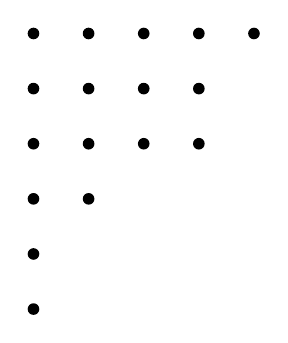
\begin{tikzpicture}[scale=0.7]
 \fill foreach \Z [count=\Y] in {5,4,4,2,1,1}
  {foreach \X in {1,...,\Z} 
  {(\X,-\Y) circle[radius=3pt]}};

\end{tikzpicture}
\]
Youngov diagram:
\[\young(~~~~~,~~~~,~~~~,~~,~,~)\]

\begin{defn}\mbox{}\\
p(n) ... število vseh razčlenitev n\\
$p_k(n)$ ... število razčlenitev n s k členi\\
$\overline{p_k}(n)$ ... število razčlenitev n z $\leqslant$ k členi
\end{defn}

n = 0: (), p(0) = 1, $p_0$(0) = 1\\
n = 1: 1\\
n = 2: 2, 1 1\\
n = 3: 3, 2 1, 1 1 1\\
n = 4: 4, 3 1, 2 2, 2 1 1, 1 1 1 1\\
n = 5: 5, 4 1, 3 2, 3 1 1, 2 2 1, 2 1 1 1, 1 1 1 1 1\\

p(n) : 1, 1, 2, 3, 5, 7, 11, 15 ...\\
$\text{p}_2(5)$ = 2\\
$\overline{\text{p}_3}(5)$ = 5\\

\begin{defn} [Konjugirana razčlenitev $\lambda '$]\mbox{}\\
(transponiramo diagram)

\[5 \ 4 \ 4 \ 2 \ 1 \ 1 ' = 6 \ 4 \ 3 \ 3 \ 1\]
\[\lambda_i ' = |\{i: \lambda_j \geqslant i\}| = max\{j: \lambda_j \geqslant i\}\]
\[\lambda '' = \lambda\]
\[\lambda_1 ' = l(\lambda)\]
\[l(\lambda ') = \lambda_1\]

Ni lepe formule za p(n), $\text{p}_k$(n), $\overline{\text{p}_k}$(n).
\end{defn}

\begin{claim}\mbox{}\\
\begin{enumerate}
    \item $p_k(n)$ = $\overline{p_{k - 1}} (n - k)$
    \item $p_k(n)$ = $p_{k - 1} (n - 1)$ + $p_k (n - k)$
    \item $\overline{p_{k}}(n)$ = $\overline{p_{k - 1}}(n) + p_k (n)$ = $\overline{p_{k - 1}}(n) + \overline{p_k} (n - k)$ 
\end{enumerate}
\end{claim}

\begin{pro}\mbox{}\\
    \begin{enumerate}
        \item Izbrišemo / dodamo prvi stolpec / stolpec dolžine k
        \item Imamo razčlenitev n s k členi: $\lambda_l$ = 1 ($p_{k - 1}(n - 1)$) in $\lambda_l$ $\geqslant$ 2 ($p_k(n - k)$)
        \item Očitno
    \end{enumerate}
    \qed
\end{pro}

OPOMBA (do zdaj obravnavane rekurzivne formule):\\
\begin{itemize}
    \item $\binom{n}{k} = \binom{n - 1}{k - 1} + \binom{n - 1}{k}$
    \item c(n, k) = c(n - 1, k - 1) + (n - 1) c(n - 1, k)
    \item S(n, k) = S(n - 1, k - 1) + k S(n - 1, k)
    \item L(n, k) = L(n - 1, k - 1) + (n + k - 1) L(n - 1, k)
    \item $p_k$(n) = $p_{k - 1}$(n - 1) + $p_k$ (n - k)
    \item $\overline{p_k}$(n) = $\overline{p_{k - 1}}$(n) + $\overline{p_k}$(n - k)
\end{itemize}

$p_k$(n):\\
\begin{tabular}{c|c c c c c c c|c}
    n $\setminus$ k & 0 & 1 & 2 & 3 & 4 & 5 & 6 & $\sum_k p_k(n)$ = p(n) \\
    \hline
    0 & 1 & 0 & 0 & 0 & 0 & 0 & 0 & 1 \\
    1 & 0 & 1 & 0 & 0 & 0 & 0 & 0 & 1 \\
    2 & 0 & 1 & 1 & 0 & 0 & 0 & 0 & 2 \\
    3 & 0 & 1 & 1 & 1 & 0 & 0 & 0 & 3 \\
    4 & 0 & 1 & 2 & 1 & 1 & 0 & 0 & 5 \\
    5 & 0 & 1 & 2 & 3 & 1 & 1 & 0 & 7 \\
    6 & 0 & 1 & 3 & 3 & 2 & 1 & 1 & 11 \\
\end{tabular}\\

POSTOPEK ZA IZPOLNITEV TABELE: Diagonalni elementi so enice, ko je k > n (nad diagonalo) so ničle, v prvem stolpcu so ničle, ostali so izračunani z rekurzivno formulo $p_k$(n) = $p_{k - 1}$(n - 1) + $p_k$ (n - k).

%\begin{itemize}
%    \item $p_n$(n) = 1 (diagonalni elementi so enice)
%    \item $p_k$(n) = 0, k > n (elementi nad diagonalo so 0)
%    \item $p_1$(n) = n, n $\geqslant$ 1
%    \item $p_2$(n) = $\lfloor \frac{n}{2} \rfloor$
%    \item $\overline{p_n}$(n) = p(n)
%\end{itemize}

Kaj pa rekurzija za p(n)?\\
A = {razčlenitve n} = $\displaystyle \bigcup_{i = 1}^n A_i$\\
$A_i$ = {razčlenitve n, ki vsebujejo i kot člen}\\
\[|A_i| = p(n - i)\]
\[|A_i \bigcap_{i \neq j} A_j| = p(n - i - j)\]
\[|A_I| = p(n - \sum_{i \in I} i)\]

\begin{align}
	|\bigcup_{i = 1}^n A_i| = & |A_1| + ... + |A_n|\nonumber\\
    			& - |A_1 \bigcap A_2| - |A_1 \bigcap A_3| ...\nonumber\\
                & + |A_1 \bigcap A_2 \bigcap A_3| ...\nonumber\\
                & - ...\nonumber\\
                & + ...\nonumber
\end{align}

\begin{align}
	p(n) = & p(n - 1) + p(n - 2) + \cancel{p(n - 3)} + \cancel{p(n - 4)} + \cancel{p(n - 5)} + ...\nonumber\\
    	& - \cancel{p(n - 1 - 2)} - \cancel{p(n - 1 - 3)} - \cancel{p(n - 2 - 3)} - \underline{p(n - 1 - 4)} - ...\nonumber\\
        & + p(n - 1 - 2 - 3) + p(n - 1 - 2 - 4) + ...\nonumber\\
        & - p(n - 1 - 2 - 3 - 4) - ...\nonumber\\
        & + ...\nonumber
\end{align}

Torej očitno: p(n) = $\displaystyle\sum_{m=1}^{\infty}$ ? p(n - m)\\
Relevantne so razčlenitve m z različnimi členi
\[7 = 7 = 6 + 1 = 5 + 2 = 4 + 3 = 4 + 2 + 1\]
$\alpha$(m) ... število razčlenitev m z lihomnogo različnimi členi\\
$\beta$(m) ... število razčlenitev m z sodo mnogo različnimi členi\\
p(n) = $\sum_{m = 1}^{\infty} (\alpha(m) - \beta (m)$ p(n - m)

\begin{claim}
\[\alpha(m) - \beta(m) = \begin{cases}(-1)^{k - 1}: \quad m = \frac{k (3k \pm 1)}{2}  \\ 0: \quad sicer \end{cases}\]
\[\frac{k (3k - 1)}{2}: 1, 5, 12, 22, ...\]
\[\frac{k (3k + 1)}{2}: 2, 7, 15, 26, ...\]
\end{claim}

Posledica: (Eulerjev petkotniški izrek)\\
p(n) = p(n - 1) + p(n - 2) - p(n - 5) - p(n - 7) + p(n - 12) + p(n - 15) - p(n - 22) - p(n - 26) ...\\
p(n) = $\displaystyle\sum_{k = 1}^{\infty} (-1)^{k - 1} (p(n - \frac{k (3k - 1)}{2}) + p(n - \frac{k (3k + 1)}{2}))$

\begin{pro}[Dokaz trditve]\mbox{}\\
Iščemo 'skoraj bijekcijo'\\
\[\{\text{razčlenitve m z liho mnogo členi}\} \iff \{\text{razčlenitve m z sodo mnogo členi}\}\]
m = 10:\\
% poskusi polepšati
\mbox{}\\


%\begin{align*}
%    \vspace{0pt}
%    \begin{tikzpicture}[scale=0.5] % prva vrstica
%        \fill foreach \Z [count=\Y] in {10}
%          {foreach \X in {1,...,\Z} 
%          {(\X,-\Y) circle[radius=5pt]}};
%    \end{tikzpicture}
%    &\iff
%    \vspace{0pt}
%    \begin{tikzpicture}[scale=0.7]
%        \fill foreach \Z [count=\Y] in {9, 1}
%          {foreach \X in {1,...,\Z} 
%          {(\X,-\Y) circle[radius=3pt]}};
%    \end{tikzpicture}
%\\\mbox{}\\
%    \begin{tikzpicture}[scale=0.7]% druga vrstica
%        \fill foreach \Z [count=\Y] in {7, 2, 1}
%          {foreach \X in {1,...,\Z} 
%          {(\X,-\Y) circle[radius=3pt]}};
%    \end{tikzpicture}
%    &\iff
%    \begin{tikzpicture}[scale=0.7]
%        \fill foreach \Z [count=\Y] in {8, 2}
%          {foreach \X in {1,...,\Z} 
%          {(\X,-\Y) circle[radius=3pt]}};
%    \end{tikzpicture}
%\\\mbox{}\\
%    \begin{tikzpicture}[scale=0.7]% tretja vrstica
%        \fill foreach \Z [count=\Y] in {6, 3, 1}
%          {foreach \X in {1,...,\Z} 
%          {(\X,-\Y) circle[radius=3pt]}};
%    \end{tikzpicture}
%    &\iff
%    \begin{tikzpicture}[scale=0.7]
%        \fill foreach \Z [count=\Y] in {7, 3}
%          {foreach \X in {1,...,\Z} 
%          {(\X,-\Y) circle[radius=3pt]}};
%    \end{tikzpicture}
%\\\mbox{}\\
%    \begin{tikzpicture}[scale=0.7]% četrta vrstica
%        \fill foreach \Z [count=\Y] in {5, 4, 1}
%          {foreach \X in {1,...,\Z} 
%          {(\X,-\Y) circle[radius=3pt]}};
%    \end{tikzpicture}
%    &\iff
%    \begin{tikzpicture}[scale=0.7]
%        \fill foreach \Z [count=\Y] in {6, 4}
%          {foreach \X in {1,...,\Z} 
%          {(\X,-\Y) circle[radius=3pt]}};
%    \end{tikzpicture}
%\\\mbox{}\\
%    \begin{tikzpicture}[scale=0.7]% peta vrstica
%        \fill foreach \Z [count=\Y] in {5, 3, 2}
%          {foreach \X in {1,...,\Z} 
%          {(\X,-\Y) circle[radius=3pt]}};
%    \end{tikzpicture}
%    &\iff
%    \begin{tikzpicture}[scale=0.7]
%        \fill foreach \Z [count=\Y] in {4, 3, 2, 1}
%          {foreach \X in {1,...,\Z} 
%          {(\X,-\Y) circle[radius=3pt]}};
%    \end{tikzpicture}
%\end{align*}














\[
\begin{tikzpicture}[scale=0.7] % prva vrstica
 \fill foreach \Z [count=\Y] in {10}
  {foreach \X in {1,...,\Z} 
  {(\X,-\Y) circle[radius=3pt]}};

\end{tikzpicture} \iff  
\begin{tikzpicture}[scale=0.7]
 \fill foreach \Z [count=\Y] in {9, 1}
  {foreach \X in {1,...,\Z} 
  {(\X,-\Y) circle[radius=3pt]}};

\end{tikzpicture}\]

\[\begin{tikzpicture}[scale=0.7]% druga vrstica
 \fill foreach \Z [count=\Y] in {7, 2, 1}
  {foreach \X in {1,...,\Z} 
  {(\X,-\Y) circle[radius=3pt]}};

\end{tikzpicture} \iff  
\begin{tikzpicture}[scale=0.7]
 \fill foreach \Z [count=\Y] in {8, 2}
  {foreach \X in {1,...,\Z} 
  {(\X,-\Y) circle[radius=3pt]}};

\end{tikzpicture}\]

\[
\begin{tikzpicture}[scale=0.7]% tretja vrstica
 \fill foreach \Z [count=\Y] in {6, 3, 1}
  {foreach \X in {1,...,\Z} 
  {(\X,-\Y) circle[radius=3pt]}};

\end{tikzpicture} \iff 
\begin{tikzpicture}[scale=0.7]
 \fill foreach \Z [count=\Y] in {7, 3}
  {foreach \X in {1,...,\Z} 
  {(\X,-\Y) circle[radius=3pt]}};

\end{tikzpicture}\]

\[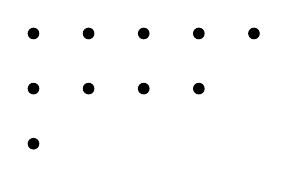
\begin{tikzpicture}[scale=0.7]% četrta vrstica
 \fill foreach \Z [count=\Y] in {5, 4, 1}
  {foreach \X in {1,...,\Z} 
  {(\X,-\Y) circle[radius=3pt]}};

\end{tikzpicture} \iff  
\begin{tikzpicture}[scale=0.7]
 \fill foreach \Z [count=\Y] in {6, 4}
  {foreach \X in {1,...,\Z} 
  {(\X,-\Y) circle[radius=3pt]}};

\end{tikzpicture}\]

\[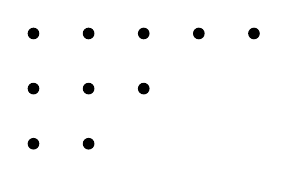
\begin{tikzpicture}[scale=0.7]% peta vrstica
 \fill foreach \Z [count=\Y] in {5, 3, 2}
  {foreach \X in {1,...,\Z} 
  {(\X,-\Y) circle[radius=3pt]}};

\end{tikzpicture} \iff 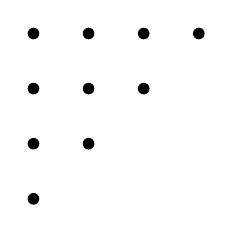
\begin{tikzpicture}[scale=0.7]
 \fill foreach \Z [count=\Y] in {4, 3, 2, 1}
  {foreach \X in {1,...,\Z} 
  {(\X,-\Y) circle[radius=3pt]}};

\end{tikzpicture}\]

s($\lambda$) $\coloneqq$ $\lambda_{l(\lambda)}$ najmanjši člen
\[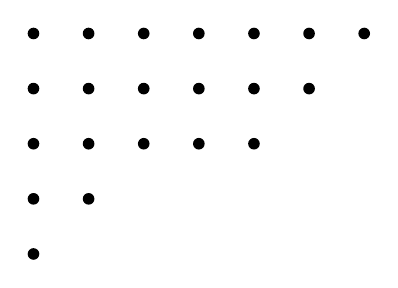
\begin{tikzpicture}[scale=0.7]
 \fill foreach \Z [count=\Y] in {7, 6, 5, 2, 1}
  {foreach \X in {1,...,\Z} 
  {(\X,-\Y) circle[radius=3pt]}};
\end{tikzpicture}\]
Recimo diagonali, ki se pojavi ob koncu prvih treh vrstic, \textbf{bok}.\\
\[b(\lambda) \coloneqq max\{i: \lambda_i = \lambda_1 - i + 1\}\]

\begin{enumerate}
    \item Če je s($\lambda$) > b($\lambda$): bok postavimo pod najmanjši člen
    \item Če je s($\lambda$) $\leqslant$ b($\lambda$): najmanjši člen postavimo desno od boka
\end{enumerate}

Zakaj to ni vselej bijekcija?\\
(dodaj sliko)\\
Prvo pravilo ne deluje, če
\[b(\lambda) = l(\lambda) = s(\lambda) - 1 = k\]
% Dodaj sliko
\[(k + 1) + (k + 2) + ... + (k + k) =\]
\[\frac{2k (2k + 1)}{2} - \frac{k (k + 1)}{2} = \frac{k (3k + 1)}{2}\]
Drugo pravilo ne deluje, če
\[b(\lambda) = l(\lambda) = s(\lambda) = k\]
% Dodaj sliko
\[k + (k + 1) + (k + 2) + ... + (k + k - 1) =\]
\[\frac{(2k - 1) 2k}{2} - \frac{(k - 1) k}{2} = \frac{k (3k - 1)}{2}\]

Torej:\\
\begin{itemize}
    \item če m $\neq$ $\frac{k (3k \pm 1}{2}$, smo našli bijekcijo, $\alpha$(m) - $\beta$(m) = 0.
    \item če m = $\frac{k (3k \pm 1}{2}$, imamo biječcijo, če odstavimo eno razčlenitev s k členi.\\
    k sod: $\alpha$(m) - $\beta$(m) = -1\\
    k lih: $\alpha$(m) - $\beta$(m) = 1\\
    Torej: $\alpha$(m) - $\beta$(m) = $(-1)^{k - 1}$
\end{itemize}
\qed
\end{pro}

OPOMBA: (dodaj sliko petkotnikov)\\

\subsection{Dvanajstera pot}
Imamo n kroglic in k škatel. Zanimajo nas razporeditve teh kroglic v škatle, torej preslikave:
\begin{itemize}
    \item injektivna preslikava: v vsaki škatli je največ ena kroglica
    \item surjektivna preslikava: v vsaki škatli je vsaj ena kroglica
\end{itemize}
Zanima nas tudi, če med sabo ločimo kroglice in škatle.
\[\begin{tabular}{c|c|c c c}
    N & K & vse & injektivne & surjektivne \\
\hline
    L & L & $k^n$ & $k^{\underline{n}}$ & k! s(n, k)\\
    N & L & $\binom{n + k - 1}{k - 1}$ & $\binom{k}{n}$ & $\binom{n - 1}{k - 1}$\\
    L & N & $\displaystyle\sum_{i \leqslant k}$ s(n, i) & $\begin{cases}1: \quad k \geqslant n  \\ 0: \quad sicer \end{cases}$ & s(n, k)\\
    N & N & $\overline{p_k}(n)$ & $\begin{cases}1: \quad k \geqslant n  \\ 0: \quad k < n \end{cases}$ & $p_k$(n) \\
\end{tabular}\]


% 16. 11. 2021

1. vrstica: šteje preslikave\\
2. vrstica: f, g: \{1, 2, 3\} $\rightarrow$ \{a, b, c, d\}
\[f: \frac{1, 2}{a} \ \frac{}{b} \ \frac{3}{c} \ \frac{}{d}\]
\[g: \frac{1, 3}{a} \ \frac{}{b} \ \frac{2}{c} \ \frac{}{d}\]
\[\text{Velja, da sta f $\sim_N$ g za ekvivalentno relacijo:}\]
\[f \sim_N g \text{, če $\exists$ } \pi \in S(n)\text{, da je f = g} \circ \pi\]
3. vrstica: $f \sim_K g$, če $\exists$ $\sigma$ $\in$ S(K), $f = \sigma \circ g$\\
4. vrstica: $f \sim_{N, K} g$, če $\exists$ $\pi$ $\in$ S(N), $\exists$ $\sigma$ $\in$ S(K), $f = \sigma \circ g \circ \pi$\\

\section{Rodovne funkcije}
\subsection{Uvod}
Zaporedja:
\[\begin{tabular}{c c c}
    $a_n = 2^n$ & $b_n = n!$ & $F_n$ Fibonaccijeva števila
\end{tabular}\]
Kako lahko 'predstavimo' zaporedje?
\begin{enumerate}
    \item Z eksplicitno formulo\\
    \[\begin{tabular}{c c c}
    $a_n = 2^n$ & $b_n = n!$ & $F_n = \frac{1}{\sqrt{5}}((\frac{1 + \sqrt{5}}{2})^{n + 1} - (\frac{1 - \sqrt{5}}{2})^{n + 1})$
    \end{tabular}\]
    \item Z rekurzivno zvezo\\
    \[a_n = F_{n \geqslant d} (a_{n - 1}, a_{n - 2}, ...)\text{ + začetni členi }a_0, ... a_{d - 1}\]
    
    % POPRAVI !!!
    
    \begin{tabular}{c c c}
    $a_n = 2a_{n-1}, \ a_0 = 1$ & $b_n = nb_{n - 1}, \ n \geqslant 1, \ b_0 = 1$ & $F_n = F_{n - 1} + F_{n - 2}, \ n \geqslant 2, \ F_0 = 1, \ F_1 = 1$
    \end{tabular}
    
    \item Z asimptotsko formulo\\
    \[a_n \sim b_n\] \[(a_n \text{ je asimptotsko enako preprostejšemu }b_n)\]
    po definiciji:\[\lim_{n \to \infty} \frac{a_n}{b_n} = 1\]
    Primer:
    \[F_n \sim \frac{1}{\sqrt{5}}(\frac{1 + \sqrt{5}}{2})^{n + 1}\]
    \[n! \sim \sqrt{2 \pi n}(\frac{n}{e})^n\]
    Tipično: $a_n \sim A n^B C^n$
    \[2^{64} = (((((2^2)^2)^2)^2)^2)^2\]
    \[2^{100} = ((2^{24}2)^2)^2\]
    Potence računamo v logaritmu eksponenta (število operacij). n! je počasno.
    \item Z rodovno funkcijo\\
    \[\sum_{n=0}^{\infty} 2^n x^n = \frac{1}{1 - 2x}, \ (|x| < \frac{1}{2})\]
    Zaporedje ''zakodiramo'' v funkcijo
    \[\sum_{n = 0}^{\infty} n! x^n\]
    Spomnimo se iz analize: $\sum_{n = 0}^{\infty} a_n x^n$ je potenčna vrsta in konvergira na (-R, R), kjer je R konvergenčni polmer, divergira pa na (-$\infty$, -R) $\bigcup$ (R, $\infty$), v x = $\pm$ R konvergira ali divergira.
    \[R = \lim_{n \to \infty} |\frac{a_n}{a_{n + 1}}| \text{, če limita obstaja}\]
    \[R = \frac{1}{\limsup\limits_{n \to \infty} \sqrt[n]{|a_n|}} \in [0, \infty)\]
    Za $\sum_{n = 0}^{\infty} a_n z^n$, z $\in$ $\C$ velja podobno: konvergira za |z| < R, divergira za |z| > R.
    \begin{itemize}
        \item $\sum_{n = 0}^{\infty} 2^n x^n$, R = $\lim_{n \to \infty} (\frac{2^n}{2^{n + 1}}) = \frac{1}{2}$, $\frac{1}{\limsup\limits_{n \to \infty} \sqrt[n]{|2^n|}} = \frac{1}{2}$
        \item $\sum_{n = 0}^{\infty} n! x^n$, R = $\lim_{n \to \infty} (\frac{n!}{(n + 1)!}) = 0$, divergira za x $\neq$ 0,  $e^x$ = $\sum_{n = 0}^{\infty} \frac{1}{n!} x^n$
    \end{itemize}
    Drugače:
    \begin{itemize}
        \item $\sum_{n = 0}^{\infty} a_n x^n$ je (običajna) rodovna funkcija $(a_n)_n$
        \item $\sum_{n = 0}^{\infty} \frac{a_n}{n!} x^n$ je eksponentna rodovna funkcija $(a_n)_n$
    \end{itemize}
    \[\sum_{n = 0}^{\infty} \frac{n!}{n!} = \frac{1}{1 - x}\]
    \[\sum_{n = 0}^{\infty} \frac{2^n}{n!} = e^{2x}\]
\end{enumerate}

\subsection{Formalne potenčne vrste}
Polinomi: realni($\R$[x]) / kompleksni($\C$[x])
\[\R [x] = \{a_0 + a_1 x + a_2 x^2 + ... + a_n x^n: a_0, ..., a_n \in \R\}\]
\[\sum_{i = 0}^n a_i x^{i} + \sum_{j = 0}^m b_j x^j = \sum_{i = 0}^{max(n, m)}(a_i + b_i)x^{i}\]
\[(a_i = 0: i > n; b_j = 0, j > m)\]
Druga definicija:
\[\R[x] = \{(a_0, ..., a_n): a_n \in \R. le končno mnogo a_n \neq 0\}\]
realna zaporedja = $\R^{\N}$

\[\lambda_{\lambda \in \R} (a_0 + a_1 x + ... + a_n x^n) = \lambda a_0 + \lambda a_1 x + ... + \lambda a_n x^n\]

($\R$[x], +, $\cdot$) je (neskončnorazsežen) vektorski prostor (za $\cdot$ množenje s skalarjem)\\
$\R_n$[x] = \{$a_0 + a_1 x + ... + a_n x^n: a_0, ..., a_n \in \R$\} polinomi stopnje $\leqslant$ n vektorski prostor ((n + 1) - dimenzionalen)
\begin{itemize}
    \item[] $1, x, x^2, ..., x^n \text{ ... standardna baza } \R_n[x]$
    \item[] $1, x^{\underline{1}}, x^{\underline{2}}, ..., x^{\underline{n}}$ in $1, x^{\overline{1}}, x^{\overline{2}}, ..., x^{\overline{n}}$ tudi bazi
\end{itemize}

\[\sum_k c(n, k) x^n = x^{\overline{n}}\]
[c(n, k)] prehodna matrika
\[\sum_k S(n, k) x^{\overline{n}} = x^n\]

$(a_0 + a_1 x + ... + a_n x^n)(b_0 + b_1 x + ... + b_m x^m) = a_0 b_0 + (a_0 b_1 + a_1 b_0)x + (a_0 b_2 + a_1 b_ 1 + a_2 b_0) x^2 + (a_0 b_3 + a_1 b_2 + a_2 b_1 + a_3 b_0)x^3 + ... + a_n b_m x^{n + m}$

Koeficienti pri $x^k$: $a_0 b_k + a_1 b_{k - 1} + ... + a_k b_0$ = $\displaystyle\sum_{i = 0}^k a_i b_{k - i}$ = $\displaystyle\sum_{\substack{i, j \geqslant 0 \\ i + j = k}} a_i b_j$
Temu rečemo konvolacijsko množenje\\
($\R$[x], +, $\cdot$) komutativen kolobar (za $\cdot$ množenje polinomov)\\
$\R$[x], z vsemi temi operacijami, je komutativna algebra ($\R^{n \times n}$ nekomutativna algebra, C([0, 1]) komutativna algebra)

\begin{defn}\mbox{}\\
    Algebra formalnih potenčnih vrst $\R$[[x]]:
    elementi so zaporedja v $\R$.
    \[\R[[x]] = \{(a_0, a_1, a_2, ...): a_i \in \R\} = \R^{\N}\]

    \[(a_n)_n + (b_n)_n = (a_n + b_n)_n\]
    \[\lambda(a_n)_n = (\lambda a_n)_n\]
    \[(a_n)_n (b_n)_n = (\sum_{k = 0}^n a_k b_{n - k})_n\]
    \[\R[[x]] \text{ komutativna algebra in } \R[x] \text{ podalgebra}\]

    OZNAKA: namesto $(a_n)_n$ ali $a_0$, $a_1$, $a_2$, ... pišemo $\displaystyle \sum_{n = 0}^{\infty} a_n x^n$ oziroma $a_0 + a_1 x + a_2 x^2 + ...$\\

    V tem primeru x ni spremenljivka, $x^n$ ni potenciranje, $\cdot$ ni množenje in + ni seštevanje $\rightarrow$ so samo oznaka.\\
    \[(a_0 + a_1 x + a_2 x^2 + ...) (b_0 + b_1 x + b_2 x^2 + ...) = a_0 b_0 + (a_0 b_1 + a_1 b_0)x + ...\]
    Enota za množenje:
    \[1 + 0 x + 0 x^2 + ... = 1\]
    Velja tudi
    \[(1 + x + x^2 + ...) (1 - x) = 1\]
    torej sta $(1 + x + x^2 + ...)$ in $(1 - x)$ inverzna za množenje.
    \[\sum_{n = 0}^{\infty} x^n = \frac{1}{1 - x}\]
\end{defn}

\begin{claim}
    \[F(x) = \sum_{n = 0}^{\infty} a_n x^n \text{ ima inverz za množenje } \iff a_0 \neq 0\]
\end{claim}

\begin{pro}\mbox{}\\
    ($\Longrightarrow$)\\
    \[\sum_{n = 0}^{\infty} a_n x^n \cdot \sum_{n = 0}^{\infty} b_n x^n = 1\]
    \begin{align*}
        a_0 b_0 &= 1\\
        a_0 b_1 + a_1 b_0 &= 0\\
        a_0 b_2 + a_1 b_1 + a_2 b_0 &= 0\\
        ... &= 0
    \end{align*}
    
    ($\Longrightarrow$)\\
    Skonstruiramo inverz G(x) = $\displaystyle \sum_{n = 0}^{\infty} b_n x^n$
    \begin{align*}
        b_0 &= \frac{1}{a_0}\\
        b_1 &= -\frac{a_1 b_0}{a_0}\\
        b_2 &= - \frac{a_1 b_1 + a_2 b_0}{a_0}\\
        &...
    \end{align*}
    \qed
\end{pro}
OZNAKE:
\begin{itemize}
    \item[] F(x) = $\displaystyle \sum_{n = 0}^{\infty} a_n x^n$
    \item[] [$x^n$]F(x) $\coloneqq$ $a_n$
    \item[] f(0) $\coloneqq$ [$x^0$]F(x) ($\cancel{\text{F(1)}}$, $\cancel{\text{F(}\frac{1}{2}\text{)}}$ $\implies$ samo F(0) - začetna vrednost) 
    \item[] (F $\cdot$ G)(0) = F(0) $\cdot$ G(0)
    \item[] Iz analize: f(x) = $\lim_{h \to 0} \frac{f(x + h) - f(x)}{h}$
    \item[] V $\R$[[x]] to ni smiselno
\end{itemize}

\begin{defn}[Odvajanje]
    \begin{align*}
        F(x) &= \sum_n a_n x^n\\
        F'(x) &\coloneqq \sum_n (n + 1) a_{n + 1} x^n\\
        (a_0, a_1, a_2, ...) &\longmapsto (a_1, 2a_2, 3a_3, ...)\\
        (F(x) G(x))' &= F'(x) G(x) + F(x) G'(x)
    \end{align*}
\end{defn}

\begin{pro}\mbox{}\\
    Gledamo [$x^n$]\\
    L: $(n + 1) (a_0 b_{n + 1} + a_1 b_n + ... + a_{n + 1} b_0)$\\
    D: $a_1 b_n + 2a_2 b_{n - 1} 3a_3 b_{n - 2} + ... + (n + 1) a_{n + 1} b_0$\\
    $+ a_0 (n+1) b_{n+1} + a_1 n b_{n} + a_2 (n-1) b_{n-1} + ... + a_n b_1 = $\\
    $= (0+n+1)(a_0 b_{n+1}) + (1+n)(a_1 b_n) + (2+n-1)(a_2 b_{n-1}) + ... +$ \\
    $+ (n+1)(a_n b_1) + (n+1+0)(a_{n+1} b_0)$ 
    \qed
\end{pro}

\begin{defn}
    \[e^{\lambda x} \coloneqq \sum_n \frac{\lambda^n}{n!} x^n\]
    \[\text{Velja } e^{\lambda x} \cdot e^{\mu x} = e^{(\lambda + \mu) x}\]
\end{defn}

\begin{pro}
    \[\sum_{k = 0}^{n} \frac{\lambda^k}{k!} \frac{\mu^{n - k}}{(n - k)!} ?= \frac{(\lambda + \mu)^n}{n!}\]
    Če zgornjo enačbo delimo z n!, dobimo
    \[\sum_{k = 0}^{n} \binom{n}{k} \lambda^k \mu^{n - k} = (\lambda + \mu)^{n}\]
    kar pa je res po binomskem izreku.
    \qed
\end{pro}

OPOMBA:\\
Imamo tudi $\C$[[x]] in $\Q$[[x]]\\
Splošneje: K[[x]], k komutativen obseg (= polje (= field))\\
(K, +) abelova grupa, (K $\setminus$ \{0\}, $\cdot$) abelova grupa in velja distributivnost.\\
Končna polja: npr. $\Z_p$, p praštevilo.

\begin{theorem}\mbox{}\\
    Polje velikosti n obstaja natanko tedaj, ko je n potenca praštevila (n = $n^p$). To polje je do izomorfizma samo eno.
\end{theorem}

V $\Z_5$: 1 + 1 + 1 + 1 + 1 = 0. $\Z_5$ ima karakteristiko 5. Končna polja imajo karakteristiko p, če so velikosti $p^k$.\\
Obseg ima karakteristiko 0, če 1 + 1 + ... + 1 $\neq$ 0 ($\Q$, $\R$, $\C$).\\
\[\text{V } \Z_5: 5! = 6! = ... = 0\]
V obsegu s karakteristiki > 0 $\frac{1}{n!}$ ni nujno definiran. Zato se omejimo na obsege s karakteristiko 0.

% 23. 11. 2021
\subsection{Uporaba rodovnih funkcij pri reševanju rekurzivnih enačb}
OPOMBA: Dejanski primeri v tem poglavju niso vključeni.\\
Parcialni ulomki:
\begin{itemize}
    \item[] Pri analizi:
    \[\int \frac{x + 1}{(2x-1)(x-1)} dx = \int (\frac{A}{2x - 1} + \frac{B}{x - 1}) dx\]
    \item[] Pri kombinatoriki:
    \[\underline{\frac{1 + x}{1 - 3x + 2x^2}} = \underline{\frac{1 + x}{(1 - 2x) (1 - x)} = \frac{A}{1 - 2x} + \frac{B}{1 - x}}\]
    \item[] Drugi način: podčrtano enakost pomnožimo z (1 - 2x) in vstavimo $x = \frac{1}{2}$. Dobimo A = 3. Pomnožimo z (1 - x) in vstavimo x = 1. Dobimo B = -2.
    \[F(x) = \frac{3}{1 - 2x} - \frac{2}{1 - x}\]
    \[a_n = 3 \cdot 2^n - 2\]
\end{itemize}

\begin{itemize}
    \item[] Pri analizi:
    \[ax^2 + nx + c = a (x - x_1)(x - x_2), \ x_{1, 2} = \frac{- b \pm \sqrt{b^2 - 4ac}}{2a}\]
    \item[] Pri kombinatoriki:
    \[c + bx + ax^2 = c(1 - y_1 x)(1 - y_2 x)\]
    kjer sta $\frac{1}{y_1}$, $\frac{1}{y_2}$ ničli $c + bx + ax^2$.
    \[c + b\frac{1}{y} + a\frac{1}{y^2} = 0 \  \ / \cdot y^2\]
    \[a + by + cy^2 = 0\]
    $y_{1, 2}$ sta torej ničli obratnega polinoma.\\
\end{itemize}

\begin{claim}
    \[\frac{1}{(1 - x)^k} = \sum_{n = 0}^{\infty} \binom{n + k - 1}{k - 1} x^n\]
\end{claim}

\begin{pro}
    \[\frac{1}{1 - x} \cdot \frac{1}{1 - x} \cdot ... \cdot \frac{1}{1 - x} = (1 + x + x^2 + ...)(1 + x + x^2 + ...)...(1 + x + x^2 + ...)\]
    \[\text{(tako na levi kot na desni strani je k členov)}\]
    Če pogledamo primer k = 3, [$x^5$]:
    \[x^5 \cdot x^0 \cdot x^0\]
    \[x^3 \cdot x^1 \cdot x^1\]
    \[x^1 \cdot x^2 \cdot x^2\]
    Dobimo šibke kompozicije.
    \qed
\end{pro}

\begin{pro}[Dokaz z indukcijo]\mbox{}\\
    Dokaz z indukcijo je bralcu prepuščen za vajo.
    \qed
\end{pro}

\[\frac{1}{1 - x} = \sum_n x^n\]
\[\frac{1}{(1 - x)^2} = \sum_n (n + 1)x^n\]
\[\frac{1}{(1 - x)^3} = \sum_n \binom{n + 2}{2} x^n\]


\begin{theorem}[recept za reševanje homogene linearne rekurzivne enačbe s konstantnimi koeficienti]
    \[c_d a_n + c_{d - 1} a_{n - 1} + ... + c_0 a_{n - d} = 0 \ \ \ n \geqslant d\]
    \[c_d \lambda^d + c_{d - 1} \lambda^{d - 1} + ... + c_0 \ \ \ (c_d, c_0 \neq 0, c_i \in \C)\]
    \[\text{(karakteristični polinom)}\]
    \[\lambda_1,... \lambda_k \text{ ničle s kratnostmi } \alpha_1, ... \alpha_k\]
    \[a_n = \sum_{i = 1}^k p_i (n) \lambda_i^n, \ \ \ \ \ deg (p_i) < \alpha_i\]
\end{theorem}

\begin{pro}
    \[c_d a_n + c_{d - 1} a_{n - 1} + ... + c_0 a_{n - d} = 0 \ \ \ / x^n / \sum_{n = d}^{\infty}\]
    \[F(x) = \sum_{n = 0}^{\infty} a_n x^n\]
    \begin{align*}
        & C_d(F(x) - a_0 - a_1x - ... - a_{d - 3}x^{d - 3} - a_{d - 2}x^{d - 2} - a_{d - 1}x^{d - 1})\\
        & + C_{d - 1} x (F(x) - a_0 - a_1x - ... - a_{d - 3}x^{d - 3} - a_{d - 2}x^{d - 2})\\
        & + C_{d - 2} x^2 (F(x) - a_0 - a_1x - ... - a_{d - 3}x^{d - 3})\\
        & + ... + c_1 x^{d - 1} (F(x) - a_0) + c_0 x^d f(x) = 0
    \end{align*}
    \[F(x) (c_d + c_{d - 1} x + c_{d - 2} x^2 + ... + c_1 x^{d - 1} + c_0 x^d) = P(x) \text{ polinom stopnje < d}\]
    \[F(x) = \frac{P(x)}{c_d + c_{d - 1} x + c_{d - 2} x^2 + ... + c_1 x^{d - 1} + c_0 x^d}\]
    Karakteristični polinom: $c_d \lambda^d + c_{d - 1} + \lambda^{d - 1} + ... + c_0$ z ničlami $\lambda_1, ..., \lambda_k$
    \begin{align*}
        F(x) & = \frac{P(x)}{c_d \prod_{i = 1}^k (1 - \lambda_i x)^{\alpha_i}} = \\
        & = \sum_{i = 1}^k \sum_{j = 1}^{\alpha_i} \frac{A_{i, j}}{(1 - \lambda_i x)^j} = \\
        & = \sum_{i = 1}^k \sum_{j = 1}^{\alpha_i} A_{i j} \sum_{n = 0}^{\infty} \binom{n + j - 1}{j - 1} \lambda_i^n x^n
    \end{align*}
    \[a_n = \sum_{i = 1}^k (\sum_{j = 1}^{\alpha_i} A_{i j} \binom{n + j - 1}{j - 1})\lambda_i^n = \sum_{i = 1}^k p_i(n)\lambda_i^n\]
    \[\binom{n  j - 1}{j - 1} = \frac{(n + j - 1)(n + j - 2) ... (n + 1)}{(j + 1)!}\]
    \[\text{ polinom stopnje (j - 1)} \implies deg(p_i) < \alpha_i\]
    \qed
\end{pro}

\begin{theorem}[Reševanje nekaterih nehomogenih rekurzivnih enačb]
    \[c_d a_n + c_{d - 1} a_{n - 1} + ... + c_0 a_{n - d} = q(n) \lambda^n\]
    Rešitev je vsota rešitve homogene enačbe in partikularne rešitve, ki jo poiščemo z nastavkom
    \[a_n = n^{\alpha} r(n) \lambda^n\]
    deg(r(n)) $\leqslant$ deg(q), $\alpha$ kratnost $\lambda$ v karakterističnem polinomu, 
    \[\alpha \geqslant 0 \text{, } \alpha = 0 \iff \lambda \text{ ni ničla}\]
\end{theorem}

\begin{pro}
    prepuščen bralcu.
\end{pro}


% 30. 11. 2021
\subsection{Binomska vrsta}

\[\binom{n}{k} = \frac{n^{\underline{k}}}{k} = \frac{n \cdot (n - 1) \cdot ... \cdot (n - k + 1)}{k!}\]
Posplošeni binomski koeficient:
\[\binom{\lambda}{n} = \frac{\lambda^{\underline{n}}}{n!} = \frac{\lambda \cdot (\lambda - 1) \cdot ... \cdot (\lambda - n + 1)}{n!}\]
$\lambda$ $\in$ K, K konvergentni obseg s karakteristiko 0, npr $\R^2$ ali $\C^2$\\
%Nekaj primerov:
\[\binom{\frac{5}{2}}{3} = \frac{\frac{5}{2} \cdot \frac{3}{2} \cdot \frac{1}{2}}{6} = \frac{5}{16}\]
\[\binom{i}{2} = \frac{i (i - 1)}{2} = \frac{-1 -i}{2}\]
\[\binom{-1}{n} \frac{(-1)(-2)...(-n)}{n!} = (-1)^n\]
k $\in$ $\N$:\\
\[\binom{-k}{n} = \frac{-k (-k - 1) ... (-k - n + 1)}{n!} = \frac{(-1)^n (n + k - 1) ... (k + 1) k}{n!} \cdot \frac{(k - 1)!}{(k - 1)!} = \]
\[ = \frac{(-1)^n (n+l+k-1)!}{n! (k - 1)!} = (-1)^n \binom{n + k - 1}{k - 1}\]

BINOMSKA VRSTA
\[B_{\lambda} (x) = \sum_{n = 0}^{\infty} \binom{\lambda}{n} x^n\]
\[= 1 + \lambda x + \frac{\lambda (\lambda - 1)}{2} x^2 + \frac{\lambda (\lambda - 1) (\lambda - 2)}{6} x^3 + ...\]
Če je $\lambda$ = n $\in$ $\N$:
\[B_n (x) = \sum_{k = 0}^{\infty} \binom{n}{k} x^k = \sum_{k = 0}^n \binom{n}{k} x^k = (1 + x)^n\]

POZOR: $B_{\lambda}$ (x) = $\displaystyle \sum_{n = 0} \binom{\lambda}{n} x^n$ je narobe! Lahko je $\displaystyle \sum_{n \in \N_0}$, $\displaystyle \sum_{n = 0}^{\infty}$ ali pa $\displaystyle \sum_{n = 0}^{\lambda}$.\\

Vemo že:
\[\frac{1}{(1 - x)^k} = \sum_{n = 0}^{\infty} \binom{n + k - 1}{k - 1} x^n\]

Za k $\in$ $\N$:
\[B_{-k} (x) = \sum_{n = 0}^{\infty} \binom{-k}{n} x^n = \sum_{n = 0}^{\infty} (-1)^n \binom{n + k - 1}{k - 1} x^n = (1 + x)^{-k}\]

Ali je smiselno $B_{\lambda} (x)$ = $(1 + x)^{\lambda}$? To je smiselno, če velja 
\[B_{\lambda} (x) \cdot B_{\mu} (x) = B_{\lambda + \mu} (x)\]

\begin{pro}\mbox{}\\
    Koeficient pri $x^n$:
    \[\sum_{k = 0}^n \binom{\lambda}{k} \binom{\mu}{n - k} \overset{?}{=} \binom{\lambda + \mu}{n}\]
    Pomnožimo z n!. Potem dokažimo
    \[(\lambda + \mu)^{\underline{n}} = \sum_{k = 0}^n \binom{n}{k} \lambda^{\underline{k}} \mu^{\underline{n - k}}\]
    z indukcijo.\\
    n = 0: 1 = 1 $\checkmark$\\
    n - 1 $\rightarrow$ n:
    \begin{align*}
        (\lambda + \mu)^{\underline{n}} & = (\lambda + \mu)^{\underline{n - 1}}(\lambda + \mu - n + 1) =\\
        & \overset{IP}{=} \sum_k \binom{n - 1}{k} \lambda^{\underline{k}} \mu^{\underline{n - 1 - k}} (\lambda - k + \mu + k - n + 1) = \\
        & = \sum_k \binom{n - 1}{k} \lambda^{\underline{k + 1}} \mu^{\underline{n - 1 - k}} + \sum_k \binom{n - 1}{k} \lambda^{\underline{k}} \mu^{\underline{n - k}} =\\
        & = \sum_k \binom{n - 1}{k - 1} \lambda^{\underline{k}} \mu^{\underline{n - k}} + \sum_k \binom{n - 1}{k} \lambda^{\underline{k}} \mu^{\underline{n - k}} = \\
        & = \sum_k \binom{n}{k} \lambda^{\underline{k}} \mu^{\underline{n - k}}
    \end{align*}
    \qed
\end{pro}

\[(1 + x)^{\lambda} \cdot (1 + x)^{\mu} = (1 + x)^{\lambda + \mu}\]
\[((x + 1)^{\frac{1}{2}})^2 = (1 + x)^{\frac{1}{2} + \frac{1}{2}} = 1 + x\]
\[((1 + x)^{\lambda})' = \lambda (1 + x)^{\lambda - 1}\]

\begin{pro}
    \[(n + 1) \binom{\lambda}{n + 1} \overset{?}{=} \lambda \binom{\lambda - 1}{n}\]
    \[\cancel{(n + 1)} \frac{\lambda^{\underline{n + 1}}}{\cancel{(n + 1)!}} = \lambda \frac{(\lambda - 1)^{\underline{n}}}{\cancel{n!}} \ \ \ \checkmark\]
\end{pro}

% ZAPISKI S TEH PREDAVANJ BODO KMALU KONČANI

% 7. 12. 2021
% by Tomaž

\subsection{Uporaba rodovnih funkcij}

(1) Rodovna funkcija je pogosto ``lepa``, tudi če za zaporedje nimamo ``lepe`` formule,
\[\text{npr. } \sum_k c(n,k)x^k = x^{\overline{n}}\] \\
(2) Rodovno funkcijo se da pogosto zapisati iz kombinatoričnega problema (več v komb 2),
npr. \[i_n \text{ število involucij v } S_n \text{, torej } \pi^2 = id \quad \sum i_n \frac{x^n}{n!} = e^{x+\frac{x^2}{2}}\]
\[\text{pomen: e na nekaj: sestavljeno iz, x: cikli dolžine 1, } \frac{x^2}{2}: \text{cikli dolžine 2}\] \\
(3) V rodovni funkciji so ``skriti`` vsi drugi zapisi zaporedja
\[\sum_n F_n x^n = \frac{1}{1-x-x^2} \to (1-x-x^2) \sum_n F_n x^n = 1\]
\[[x^n]: F_n - F_{n-1} - F_{n-2} = 0 \] \\
asimptotika: vzamemo singularnost ($x_0$), ki je najbližje izhodišču \[F_n \sim An^B(\frac{1}{x_0})^n\] \\
(4) Iz rodovnih funkcij lahko izračunamo še drugo: povprečje, varianco $\dots$ \\
npr. koliko elementov ima v povprečju podmnožica $[n]$?
\[\frac{\sum_{S \subseteq [n]} |S|}{2^n} = \frac{\sum_k k \cdot \binom{n}{k}}{2^n} = \frac{n2^{n-1}}{2^n} = \frac{n}{2}\]
\\

\section{Pólyeva teorija}

Primer: Prištejemo ogrlice s 4 koraldami in 2 barvama: ogrlici sta enaki, če eno iz druge dobimo z rotacijo.
%{\color{red} manjkajo slikice}
Splošno? \\

Kaj pa zapestnice? Zapestnici sta enaki, če eno iz druge dobimo z rotacijo ali zrcaljenjem. \\
%{\color{red} manjkajo slikice} \\


\subsection{Permutacijske grupe}

$(G, \circ)$ je grupa, če veljajo asociativnost, enota, inverz. \\
Simetrična grupa $S_n: \{\text{permutacija } [n] \to [n]\}$ \\
Permutacijska grupa: podgrupa simetrične grupe.
$H \leq G$ je podgrupa, če $e \in H$, $a,b \in H \implies a \circ b \in H$ in $a \in H \implies a^{-1} \in H$ \\
Cayleyev izrek: vsaka končna grupa je izomorfna permutacijski grupi \\
npr. ciklična grupa $C_n = \{(1 2 \dots n)^i \; \vert \; 0 \leq i \leq n-1\}$, $|C_n| = n$ \\
\[\Z_n \cong C_n \quad \cong \; \text{ pomeni izomorfnost:}\]
\[\phi: \Z_n \to C_n \quad \phi(i) = (1 2 \dots n)^i \text{ to je (očitno) izomorfizem}\]

G permutacijska grupa, $G \leq S_x$ \\
\[x \in X, \quad Gx := \{gx \; \vert \; g \in G\} \subseteq X \text{ je orbita elementa x}\]
\[X/G = \{\text{orbite}\}\]
Orbite so ekvivalenčni razredi za relacijo $\sim$, kjer \\
\[x \sim y \iff \exists g \in G: \; gx = y\]

Stabilizator \\
\[x \in X\]
\[G_x = \{g \in G \; \vert \; gx = x\} \subseteq G\]

\begin{theorem}
    \[Gx \leq G\]    
\end{theorem}

%{\color{red} za en del nism zihr a je prov}
\begin{pro}
    \[\text{id } \in G_x \text{, saj  idx } = x \; \forall x\]
    \[g,h \in G_x \implies ghx = x \implies gh \in G_x\]
    \[g \in G_x \implies g^{-1} \in G_x \; (gx = x \quad / \cdot g^{-1})\]
    \qed
\end{pro}

Opomba: $H \triangleleft G$ podgrupa edinka, če $H \leq G$ in $gHg^{-1} \subseteq H$ \\
$G_x$ v splošnem ni podgrupa edinka. \\
Spomnimo se: $H \subseteq G$, $g \in G$\\
\[gH := \{gh \vert h \in H\} \text{ levi odsek}\]
Levi odseki so disjunktni in enako močni ($eH \to gH \quad h \to gH$) \\
bijekcija $a \in gH \cap g'H \quad a=gh=g'h'$ \\
\[h,h' \in H \implies g^{-1}g' = hh'^{-1} \in H \implies g' \in gH\]
\[\implies g'H \subseteq gH \subseteq g'H \implies gH = g'H\]
\[G/H = \{\text{levi odseki}\} \quad \text{kvocientna množica}\]
Kdaj je $G/H$ grupa
\[gH \cdot g'H := gg'H\]
To je dobro definirano samo če $H \triangleleft G$ \\
Vedno: $|G/H| = \frac{|G]}{|H|}$ \\

\begin{theorem}
    \[|Gx| \cdot |G_x| = |G|\]
\end{theorem}

\begin{pro}
    Trdimo $|Gx| = \frac{|G|}{|G_x|} = |G/G_x|$ \\
    Iščemo bijekcijo $\phi: Gx \to G/G_x \quad gx \mapsto gGx$ \\
    Dokazati moramo dobro definiranost
    \[gx = g'x \; (g \neq g') \; \iff gGx = g'Gx\]
    \[gx = g'x \iff g'^{-1}gx = x \iff g'^{-1}g \in Gx \iff \]
    \[\iff g'^{-1}gGx = Gx \iff gGx = g'Gx\]
    Dokazali smo tudi injektivnost \\
    Surjektivnost: $\text{gGx } = \phi(gx)$\\
    \qed
\end{pro}



\end{document}